\section{Erläuterung Fallbeispiel}
Ziel des Fallbeispieles ist es, ein Verfahren vom Entwurf bis zur Bereitstellung von containerisierten Microservices mit Kubernetes zu implementieren. Anschließend sollen auf Basis dieses Verfahrens Aussagen zur Umsetzung und dem Anwendungsgebiet getroffen werden können. Als Beispiel wird ein vereinfachtes \ac{CRM}-System verwendet. In diesem Kapitel werden die Vorgaben an das Fallbeispiel beschrieben.

\subsection{Anwendungseinsatz}
Ein \ac{CRM}-System ist eine Software für das Kundenbeziehungsmanagement. CRM-Systeme sind komplexe betriebliche Anwendungssysteme. Durch ihre Größe und vielen verwobenen Diensten gestaltet sich der Entwurf und die Weiterentwicklung häufig schwierig. \ac{CRM}-System haben eine große fachliche Breite, was zu einem hohen Koordinationsaufwand bei der Entwicklung und Bereitstellung führt \parencite[vgl.][S. 62]{trempArchitekturen2021}. Dadurch eignet sich ein \ac{CRM}-System als gutes Beispiel für die Umsetzung mit einer Microservice-Architektur, welche die Probleme weitgehend entschärfen soll. 

Das \ac{CRM}-System soll für das \ac{B2C} Umfeld entwickelt werden. Es soll bei der Verwaltung von Kontakten beziehungsweise Kunden helfen. Zu jedem Kontakt sollen Informationen und eine Historie mit allen Interaktionen abgespeichert werden. Darüber hinaus soll es auch möglich sein Verkaufschancen zu verwalten und einem Kontakt zuzuordnen.

\subsection{Anwendungsfunktionen}
Die Kernfunktionalität des zu erstellenden \ac{CRM}-Systems ist das Anlegen, Anzeigen, Bearbeiten und Löschen von Kontakten, Interaktionen und Verkaufschancen. Konkret sollen die folgenden funktionalen Anforderungen von dem System erfüllt werden:
\begin{itemize}
\item Kontakte sollen mit Namen, Geburtsdatum, Geschlecht, Telefonnummer, E-Mail-Adresse und Adresse angelegt, angezeigt, geändert und gelöscht werden können
\item Interaktionen mit einem Kontakt sollen mit Art der Interaktion, Datum, Uhrzeit, Notizen und dem zugehörigen Kontakt angelegt, angezeigt, geändert und gelöscht werden können
\item Mögliche Verkaufschancen sollen mit Status, voraussichtlichem Abschlussdatum, Verkaufswert, Rabatt, Budget des Kunden, Notizen und dem zugehörigen Kontakt angelegt, angezeigt, geändert und gelöscht werden können
\end{itemize} 

Alle Funktionen sollen über eine sowohl über eine einfache grafische Benutzeroberfläche mit dem Webbrowser bedienbar sein, als auch über eine REST-API angesteurt werden können. Durch eine Microservice-Architektur, sollen die einzelnen Module nur lose gekoppelt sein. Dadurch soll eine flexible Skalierung und Erweiterbarkeit der Anwendung gewährleistet werden. Authentifizierung, Autorisierung und andere Sicherheitsfunktionen sollen nicht beachtet werden.

\clearpage
\section{Entwurf der Microservices}



Als Erstes wird die Architektur der Microservices festgelegt. Bei der Architektur kann zwischen Makro-Architektur und Mikro-Architektur unterschieden werden. Die Makro-Architektur befasst sich mit dem Gesamtsystem. In der Mikro-Architektur geht es um den Aufbau der einzelnen Microservices.

\subsection{Makro-Architektur}

Für die Makro-Architektur ist die genaue Umsetzung der einzelnen Microservices nicht relevant. Die Makro-Architektur ist besonders wichtig, da Veränderungen hier zu einem späteren Zeitpunkt sehr aufwendig werden können. Das Wichtigste ist die Aufteilung in Microservices nach der Fachlichkeit. Das CRM-System lässt sich in drei fachliche Bereiche unterteilen: Kontaktverwaltung, Interaktionsverwaltung und Chancenverwaltung. Die Microservices werden nach den Bereichen aufgeteilt. Jeder dieser drei bereiche Besitzt ein eigenes Datenobjekt. Das  ist ein weiterer Hinweis für eine gute Aufteilung. Die Microervices machen ihre Dienste über REST-Schnittstellen verfügbar. Für die Skalierbarkeit ist es wichtig, dass die Microservices selbst keinen zustandlos sind. Alle persistenten Daten werden in Datenbanken gehalten.

\begin{figure}[H] 
    \centering
    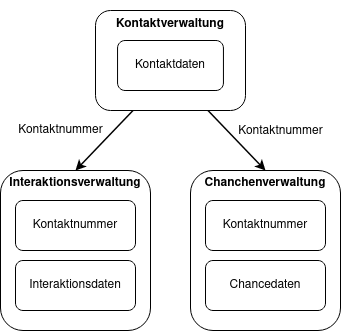
\includegraphics[width=0.71\textwidth]{figures/ContextMap.png}
    \caption{Context Map}
    \label{fig:CRMENTWURF}
\end{figure}

Alle der drei eingeteilten Microservices sollen eine eigene Datenbank erhalten. Dadurch sind die Datenschemata übersichtlich und Änderungen haben nur unmittelbare Auswirkungen auf einen Microservice. \\
\\
Das Frontend wird monolithisch Aufgebaut und integriert alle Funktionalitäten der Microservices. Das Frontend ist dadurch einheitlich. Das System könnte auch um andere Frontends erweitert werden. Das Frontend wird dabei eine clientseitige Webanwendung, welche die REST-Schnittstellen der Microservices konsumiert. \\
\\
Da sich Interaktionen und Verkaufschancen einem Kontakt bzw. Kunden zuordnen lassen sollen, ist eine Abhängigkeit zwischen diesen Microservices zu erwarten. Auch die Kommunikation zwischen Microservices soll über die gleichen REST-Schnittstellen laufen. Daraus ergibt sich der folgende Entwurf. \\
\\
\begin{figure}[H] 
    \centering
    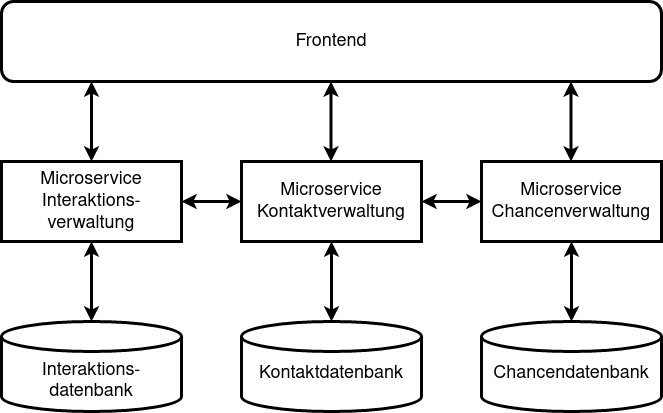
\includegraphics[width=0.71\textwidth]{figures/CRMEntwurf.png}
    \caption{Entwurf des \acp{CRM-System}}
    \label{fig:CRMENTWURF}
\end{figure}

Die REST-Schnittstellen sollten einheitlich über alle Microservices hinweg sein. Die folgende Tabelle zeigt unter welchen Endpunkten, mit welchen HTTP-Methoden und welchen Parametern die REST-APIs aufrufbar sein sollen.

\begin{table}[H]
\centering
    \begin{tabular}[H]{l|l|l|l}
        Endpunkt & HTTP-Methode & Parameter & Beschreibung \\
        \hline
        /contacts & GET & - & Gibt alle Kontakte zurück \\
        \hline
        /contacts & POST & neuer Kontakt & Fügt einen neuen Kontakt hinzu \\
        \hline
        /contacts/\{ID\} & GET & - & Gibt einen Kontakt zurück \\
        \hline
        /contacts/\{ID\} & PUT & veränderter Kontakt & Ändert einen Kontakt \\
        \hline
        /contacts/\{ID\} & DELETE & - & Löscht einen Kontakt \\
        \hline
    \end{tabular}
    \caption{Prozessoren}
\end{table}

Für das Frontend wird React verwendet. [React Erklärung]
Für alle drei Microservices wird derselbe Technologie-Stack verwendet, um den Entwicklungsaufwand geringer zu halten. Es wird Java mit dem Framework Spring Boot verwendet. Als Datenbank wird MongoDB eingesetzt. [MongoDB Erklärung] Darüber hinaus wird Swagger in die Microservices integriert. Bei Swagger handelt es sich ein Werkzeug zur sprachunabhängigen Spezifikation von APIs. Swagger kann durch eine Abhängigkeit zu Spring Boot hinzu gefügt werden. Es erstellt automatisch eine Webseite mit der Dokumentation unserer API. Um das Monitoring, Service Discovery, Load Balancing wird mit Kubernetes gelöst. Unser System muss diese Aufgaben also nicht selbst bewältigen und diese Bestandteile werden erst in der Bereitstellung konfiguriert.

\subsection{Micro-Architektur}

Die Mikro-Architektur befasst sich mit der Architektur eines einzelnen Microservice. Für das Gesamtsystem ist die Architektur eines einzelnen Microservice nicht von Bedeutung. Aus diesem Grund besitzt man eine große Freiheit bei der Auswahl. Es sollte die Architektur, welche am Simpelsten alle Anforderungen bietet. Der ausgewählte Technologie-Stack schränkt natürlich die möglichen Architekturen auch weiter ein.

Unser System besteht aus drei Microservices und einem Frontend. Das Frontend dient lediglich zur Visualisierung und Verbindung aller Funktionen der drei Microservices. Die folgenden Domänenmodelle zeigen, welche Daten von den entsprechenden Microservices verwaltet werden müssen.

\begin{figure}[H] 
    \centering
    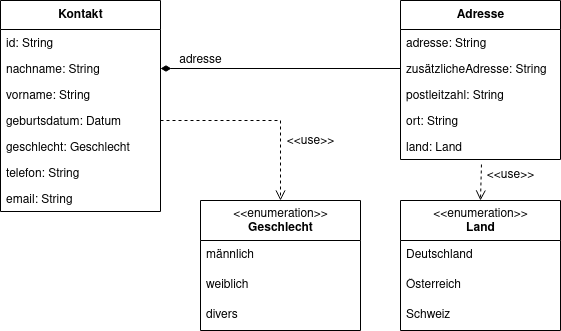
\includegraphics[width=0.71\textwidth]{figures/KontaktUMLDiagram.png}
    \caption{Context Map}
    \label{fig:CRMENTWURF}
\end{figure} 

\begin{figure}[H] 
    \centering
    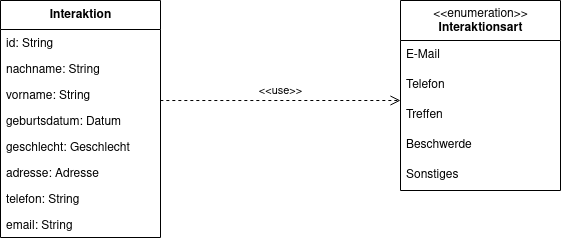
\includegraphics[width=0.71\textwidth]{figures/InteraktionUMLDiagram.png}
    \caption{Context Map}
    \label{fig:CRMENTWURF}
\end{figure} 

\begin{figure}[H] 
    \centering
    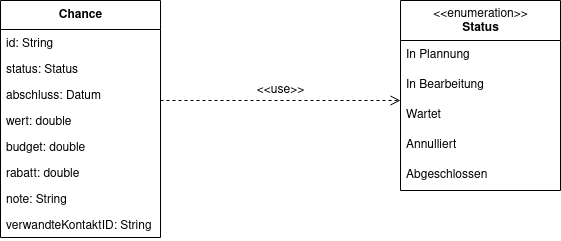
\includegraphics[width=0.71\textwidth]{figures/ChanceUMLDiagram.png}
    \caption{Context Map}
    \label{fig:CRMENTWURF}
\end{figure} 

Für die Architektur der Microservices wird eine hexagonale Architektur (Ports und Adapter) verwendet. Eine Hexagonale Architektur bietet sich 

\begin{figure}[H] 
    \centering
    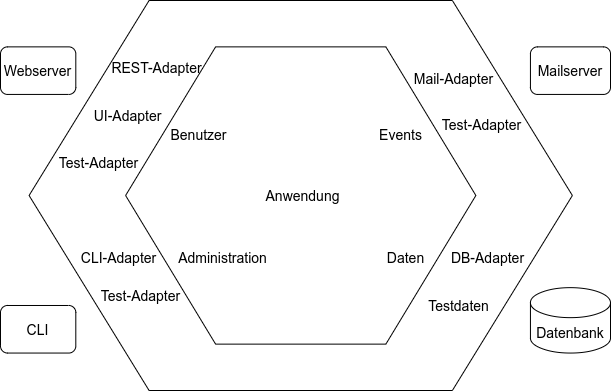
\includegraphics[width=0.71\textwidth]{figures/HexagonalDesignConcept.png}
    \caption{Entwurf des \acp{Hexagonale Architektur}}
    \label{fig:CRMENTWURF}
\end{figure}

\clearpage
\section{Implementierung}

An dieser Stelle sei auch erwähnt, dass der gesamte Quellcode im folgenden GitHub Repository einsehbar ist: \href{https://github.com/SimonHirner/bachelor-thesis}{github.com/SimonHirner/bachelor-thesis}.

In diesem Kapitel wird das CRM-System dem Entwurf nach implementiert. Als Erstes wird die Implementierung der Microservices erklärt, da alle drei durch den gleichen Technologie-Stack sehr ähnlich sind. Anschließend wird das Frontend, welches alle Microservices integriert, implementiert.

\subsection{Microservices}

Alle drei Microservices benötigen die \ac{URI} ihrer Datenbank, um mit ihr eine Verbindung aufzubauen. Der Interaktions-Microservice und der Verkaufschancen-Microservice brauchen darüber hinaus die Adresse des Kontakt-Microservices, um mit diesem zu Kommunizieren. Diese Verbindungsinformationen, werden den Anwendungen über Umgebungsvariablen übergeben. Später bei der Bereitstellung, kann mit Kubernetes den Containern die passenden Umgebungsvariablen übergeben werden.

\begin{figure}[H] 
    \centering
    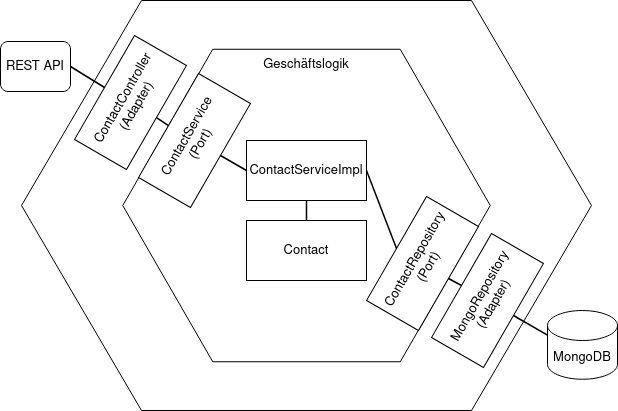
\includegraphics[width=0.71\textwidth]{figures/HexagonalDesign.png}
    \caption{Entwurf des \acp{Hexagonale Architektur}}
    \label{fig:CRMENTWURF}
\end{figure}

\begin{figure}[H] 
    \centering
    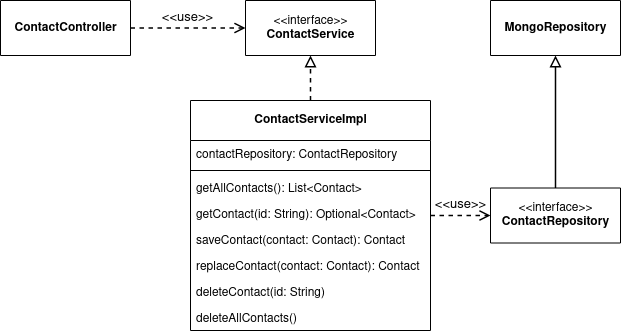
\includegraphics[width=0.71\textwidth]{figures/UMLKlassenDiagram.png}
    \caption{Entwurf des \acp{Hexagonale Architektur}}
    \label{fig:CRMENTWURF}
\end{figure}

\begin{figure}[H] 
    \centering
    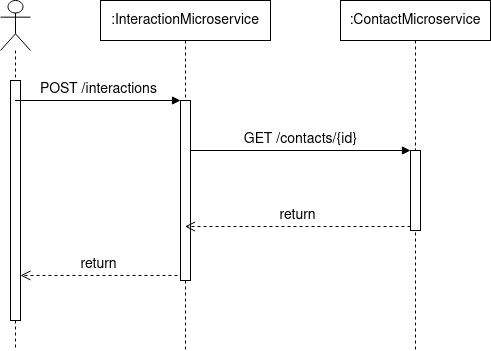
\includegraphics[width=0.71\textwidth]{figures/UMLSequenzdiagramm.png}
    \caption{Entwurf des \acp{Hexagonale Architektur}}
    \label{fig:CRMENTWURF}
\end{figure}

\subsection{Frontend}

Das Frontend. Das Frontend soll später auch mit Kubernetes bereitgestellt werden, es wird aber nicht als Microservices angesehen. Das Frontend benötigt die \ac{URI} aller Services. Auch hier werden die Verbindungsinformationen über eine Umgebungsvariable übergeben.

\clearpage
\section{Bereitstellung mit Kubernetes}

Im letzten Teil des Fallbeispiels wird das fertige CRM-System nun mit Kubernetes bereitgestellt.

\subsection{Containerisierung}

Um die Microservices und das Frontend in Pods in einem Kubernetes Cluster laufen zu lassen, müssen sie erst mit Docker containerisiert werden. Dazu wird als Erstes ein Dockerfile für jeden Microservice erstellt. Anschließend kann aus dem Dockerfile ein Docker Image gebaut werden, mit dem dann ein entsprechender Container gestartet werden kann. \\
\\

Dockerfiles besitzen eine eigene Syntax. Ein großgeschriebener Befehl wird gefolgt von einem oder mehreren Parametern. Es ist aufgebaut wie eine Anleitung, welche Schritt für Schritt abgearbeitet wird. Die Dockerfiles der Microservices haben alle den selben Aufbau, da alle drei Projekte auch die selben Aufbau und die selben Technologien verwenden. Der erste Befehl in den Dockerfiles bestimmt, auf welchem Docker Image unser eigenes Image basieren soll. Hier wird ein Image mit einer Java-Plattform verwendet, welches automatisch aus dem öffentlichen DockerHub heruntergeladen wird. Anschließend wird die JAR-Datei der Anwendung in das Image kopiert. Als letzter Befehl wird festgelegt, dass die JAR-Datei beim Start des Containers ausgeführt werden soll.

\begin{lstlisting}[language=dockerfile, caption=Dockerfile für Kontakt-Microservice]
FROM openjdk:11-jdk-slim
ARG JAR_FILE=target/*.jar
COPY ${JAR_FILE} app.jar
EXPOSE 8080
ENTRYPOINT ["java","-jar","/app.jar"]
\end{lstlisting}

Das Frontend benötigt ein eigenes Dockerfile. Dieses hat einen mehrstufigen Aufbau. Im ersten Stufe, der Build-Stage, wird unsere React-Anwendung gebaut. Um die fertig gebaute Webanwendung an einen Browser auszuliefern wird ein Webserver benötigt. In der zweiten Stufe des Dockerfiles basiert auf einem Image mit dem Webserver Nginx. Die React-Anwendung aus der Build-Stage wird nun in das finale Image kopiert.

\begin{lstlisting}[language=dockerfile, caption=Dockerfile für Frontend]
FROM node:alpine as build
WORKDIR /app
COPY package*.json ./
RUN npm install --silent
COPY . .
RUN npm run build

FROM nginx:alpine
WORKDIR /usr/share/nginx/html
RUN rm -rf ./*
COPY --from=build /app/build .
ENTRYPOINT ["nginx", "-g", "daemon off;"]
\end{lstlisting}

Für die Datenbanken müssen keine eigenen Dockerfiles erstellt werden. Hier reichen unveränderte Images, welche aus dem DockerHub heruntergeladen werden können, aus. Mit dem folgenden Befehl kann aus dem Dockerfile nun ein Docker Image gebaut werden.

\begin{lstlisting}[language=bash, caption=Befehl , captionpos=b]
docker build -t contact-microservice:latest .
\end{lstlisting}


\subsection{Bereitstellung}

Für jede Datenbank wird eine Anwendung 

\begin{figure}[H] 
    \centering
    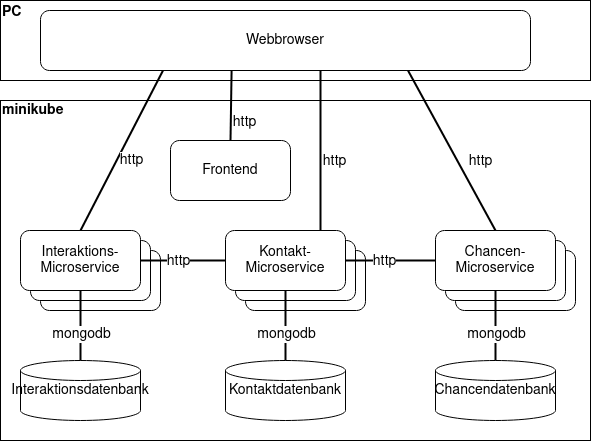
\includegraphics[width=0.71\textwidth]{figures/DeploymentDiagramm.png}
    \caption{Entwurf des \acp{Hexagonale Architektur}}
    \label{fig:CRMENTWURF}
\end{figure}

Jetzt müssen die fertigen Images in unserem Kubernetes Cluster bereitgestellt werden. Dafür werden YAML-Dateien erstellt, in denen die gewünschten Kubernetes Objekte beschrieben werden. Für jeden der drei Microservices und das Frontend muss ein Service und ein Deployment erstellt werden. Das Deployment repräsentiert die Anwendung. Mit Parametern kann festgelegt werden wie viele Pods mit der Anwendung gestartet werden sollen.

\begin{lstlisting}[language=YAML, caption=Befehl]
apiVersion: apps/v1
kind: Deployment
metadata:
  name: contact-service
spec:
  replicas: 1
  template:
    metadata:
      labels:
        app: contact-service
    spec:
      containers:
        - name: contact-service
          image: contact-microservice:latest
          imagePullPolicy: IfNotPresent
          ports:
          - containerPort: 8080
          env:
            - name: MONGODB_HOST
              valueFrom:
                configMapKeyRef:
                  name: contact-db-config  
                  key: host
\end{lstlisting}

\begin{lstlisting}[language=YAML, morekeywords=host, caption=Befehl , captionpos=b]
apiVersion: v1
kind: ConfigMap
metadata:
   name: contact-service-config
data:
 host: contact-service
\end{lstlisting}

Nach der Erstellung der Services wird die Service Discovery und Lasterverteilung von Kubernetes übernommen. 

\begin{lstlisting}[language=YAML, caption=Befehl , captionpos=b]
kind: Service
apiVersion: v1
metadata:
  name: contact-service
spec:
  selector:
    app: contact-service
  ports:
  - protocol: TCP
    port: 8080
    nodePort: 30010
  type: NodePort
\end{lstlisting}

Nun müssen nur noch alle YAML-Dateien über den folgenden kubectl-Befehl angewendet werden. Kubernetes sorg nun dafür, dass die beschriebenen Objekte, erstellt werden.

\begin{lstlisting}[language=bash, caption=Befehl , captionpos=b]
kubectl apply -f contact-microservice.yaml
\end{lstlisting}

\subsection{Skalierung}

Um die Vorteile von unseren Microservices auszunutzen, sollen die Microservices nun horizontal skaliert werden. Auch dafür wird eine YAML-Datei erstellt, in der ein HorizontalPodAutoscaler-Objekt für jeden Microservice beschrieben wird. In der Datei wird angegeben, welches Deployment skaliert werden soll. Als Metrik, wann hochskaliert werden soll, kann die CPU-Auslastung des Pods verwendet werden. Darüber hinaus wird angegeben wie viele Pods von dem entsprechenden Microservice minimal und maximal ausgeführt werden sollen.

\begin{lstlisting}[language=YAML, caption=Befehl , captionpos=b]
apiVersion: autoscaling/v1
kind: HorizontalPodAutoscaler
metadata:
    name: contact-service
spec:
    scaleTargetRef:
        apiVersion: apps/v1
        kind: Deployment
        name: contact-service
    minReplicas: 2
    maxReplicas: 4
    targetCPUUtilizationPercentage: 80
\end{lstlisting}
